% ReMSTNet manuscript draft prepared with the official MDPI LaTeX class.
% Main file for Overleaf: manuscript.tex

\documentclass[electronics,article,submit,oneauthor]{Definitions/mdpi}

%=================================================================
% MDPI metadata
\firstpage{1}
\makeatletter
\setcounter{page}{\@firstpage}
\makeatother
\pubvolume{1}
\issuenum{1}
\articlenumber{0}
\pubyear{2026}
\copyrightyear{2026}
\datereceived{}
\daterevised{}
\dateaccepted{}
\datepublished{}

% Clean author-working-copy page furniture. The MDPI `submit` option otherwise
% prints a provisional "submitted to" header, review line numbers, and a dummy
% DOI before the manuscript has entered the journal system. Remove this block
% when preparing the actual journal-submission copy.
\makeatletter
\fancypagestyle{plain}{%
  \fancyhf{}%
  \fancyfoot[C]{\fontsize{8}{8}\selectfont\thepage{} of \pageref*{LastPage}}%
  \renewcommand{\headrulewidth}{0pt}%
  \renewcommand{\footrulewidth}{0pt}%
}
\pagestyle{fancy}
\fancyhf{}
\fancyhead[R]{\fontsize{8}{8}\selectfont\thepage{} of \pageref*{LastPage}}
\renewcommand{\headrulewidth}{0pt}
\renewcommand{\footrulewidth}{0pt}
\makeatother

%=================================================================
% Local commands
\newcommand{\modelname}{ReMSTNet}
\graphicspath{{figures/}}

%=================================================================
% Front matter. Add the author's department, postal address, and ORCID before submission.
\Title{\modelname: Relation-Encoded Moment-Exact Transport for Pointer-Gauge Reading under Projective Distortion}

\Author{Xiaoyi Liang $^{1,}$*}
\AuthorNames{Xiaoyi Liang}

\address{%
$^{1}$ \quad University College London, London, UK; ucabx23@ucl.ac.uk}

\corres{Correspondence: ucabx23@ucl.ac.uk}

% Abstract: single paragraph, approximately 200 words maximum.
\abstract{Pointer gauges remain common in industry, but off-axis images alter dial support and pointer--scale relations. We present \modelname, a dual-view network that aligns raw and support-normalized features and converts bounded relation evidence into feasible first-moment updates, with exact raw-posterior fallback when geometry is undefined. The frozen foundation was fitted on 14,442 SyncG images and relation modules on a contained 6,616-image subset; no real image was used for fitting. On a retrospective 1,558-image, 14-scene benchmark, three-run NMAEs were $0.010704\pm0.000373$ across six conditions and $0.013259\pm0.000391$ in the projective pool, 23.19\% and 32.77\% below the matched support-normalized EfficientNet-B0 endpoint. On the complete 774-row same-pixel VDN intersection, \modelname\ obtained $0.008582\pm0.000414$ versus 0.016444 NMAE for an annotation-assisted VDN direction reference, a 47.81\% reduction. An organized industrial baseline of 1,395 real-photo ROIs yielded $0.123388\pm0.018553$ versus $0.123664\pm0.018317$ across six conditions; the paired interval and all three projective-condition intervals favored \modelname. A separate 153-photo full-frame diagnostic covered 151 frames. An end-to-end physical-reading replay then integrated an existing PP-OCRv4 model without OCR fitting and returned physical readings for 27/153 photos. On the 9/33 labeled photos accepted by the default range decoder, conditional NMAE was $0.036814\pm0.004015$, compared with $0.034336\pm0.003848$ using the true range on the identical accepted subset. The evidence supports selective projective transport and feasible existing-model physical-unit integration, while automatic range coverage remains a deployment bottleneck.}

\keyword{analog gauge reading; pointer meter; projective distortion; relation encoding; posterior transport; geometric validity; synthetic-data training}

%%%%%%%%%%%%%%%%%%%%%%%%%%%%%%%%%%%%%%%%%%
\begin{document}
\nolinenumbers

\section{Introduction}
\label{sec:introduction}

Analog pointer gauges remain embedded in power systems, process plants, laboratories, and legacy industrial equipment because they are inexpensive, mechanically robust, and able to operate in environments where replacing every instrument with a networked digital sensor is impractical. Visual reading offers a non-invasive route to automated inspection: a camera or mobile robot can observe an existing gauge without modifying the instrument or interrupting the monitored process. Recent systems have demonstrated mobile-phone transcription, autonomous reading in unstructured environments, and robot-deployable staged pipelines \cite{howells2021analogue,milana2022gauges,reitsma2024underpressure}. Their progress notwithstanding, reliable field reading remains difficult when a gauge is small, blurred, partly occluded, poorly illuminated, or viewed away from the dial normal.

Projective distortion is particularly consequential because it alters several coupled cues at once. An oblique view changes the apparent dial boundary, compresses angular intervals non-uniformly, modifies the foreground occupancy of a crop, and distorts the relation between the pointer and its reference scale. Established pipelines address these effects through combinations of dial detection, pointer or scale segmentation, keypoint localization, ellipse fitting, and explicit perspective correction. Tan et al. combined a TransUNet-based segmentation stage with perspective transformation correction for pointer-meter recognition \cite{tan2024transunet}. PriKMet used pointer keypoints together with inspection-route and meter-range priors to compensate for positional offsets in unmanned-aerial-vehicle inspection \cite{chu2025prikmet}. More recently, virtual points and a pose-estimation model have been used to construct a geometric rectification for strongly tilted industrial gauges \cite{lee2026p2yolo}. These studies establish the value of geometric reasoning, but they also show that ``perspective robustness'' is not a single operation: it depends on what geometry is observable, how image evidence is normalized, and how the corrected evidence is converted into a reading.

Deep gauge readers also differ in their pointer representations. Segmentation-based methods recover a mask and infer a centerline or angular position, which makes the intermediate geometry interpretable but can fail when the pointer is thin, reflective, or weakly contrasted. Vector Detection Network instead represents a pointer through a localized point and a two-dimensional direction field, thereby avoiding a full mask requirement \cite{dong2021vdn}. Other systems retain explicit stages so that detection, ellipse, needle, scale, or optical-character-recognition failures remain visible \cite{reitsma2024underpressure}. Reconstruction-based models address a different failure mode by restoring partially occluded dial content before regression \cite{ninama2026grnet}. None of these representations is uniformly preferable: each preserves certain cues and introduces characteristic failure modes. This motivates architectures that exploit complementary observations while maintaining a clearly defined fallback when their relation cannot be trusted.

Data availability compounds this problem. Real industrial gauge images are costly to collect and annotate across meter types, readings, viewpoints, and environmental conditions. Synthetic-data studies have therefore used controlled rendering to generate structural supervision and promote transfer to real images \cite{leonalcazar2023synthetic}. The recently released SyncG benchmark provides 20,000 photorealistic synthetic images across 145 environments, together with detection, keypoint, segmentation, and optical-character-recognition annotations \cite{deng2026syncg}. Such data make controlled scene-disjoint training and stress evaluation possible, but synthetic diversity does not by itself guarantee real-domain transfer. A method trained on SyncG must therefore separate same-domain gains from retrospective real-image behavior and avoid describing a synthetic test improvement as universal field robustness.

The present work starts from a narrower observation about projective inputs. A raw meter region of interest (ROI) retains the original appearance and sampling density, but a full-canvas projective transform can surround the effective dial support with large invalid or low-information regions. Support-Aware ROI Normalization (SARN-v2) deterministically identifies a valid projected support, crops it when the support geometry is reliable, and otherwise leaves the input unchanged. The raw and SARN views are consequently not treated as competing experts. They are two observations of the same gauge: one preserves the original canvas, whereas the other can restore effective object occupancy under a valid projective deformation. Simply selecting one endpoint or concatenating their final predictions would ignore where and how their intermediate evidence agrees. Moreover, because support normalization is not beneficial in every image domain, an unconstrained learned correction could replace a sound raw estimate with an unsupported one.

We therefore propose \modelname\ (Relation-Encoded Moment-Exact Transport Network), a continuous dual-view reader that embeds Raw--SARN relation modeling inside its feature hierarchy. A shared encoder processes both views. At strides 8 and 16, two ReMST blocks combine projected raw features, homography-aligned normalized features, their signed and absolute differences, multiplicative agreement, cosine similarity, and the valid support mask. Each block writes a bounded relation residual back into the raw feature stream and emits a relation memory for subsequent decoding. Thus, the second scale and the shared context are computed from features that have already been relation-conditioned; the method is not a generic classification backbone followed by an external scalar correction head.

The multi-scale memories are decoded by a progress-aware coordinator. Per-bin queries contain the two endpoint posteriors, their log probabilities and cumulative distributions, local differences, and normalized progress positions. A local depthwise mixing operator organizes evidence across neighboring progress bins. The decoder predicts one bounded total displacement and a non-negative allocation across the two relation scales and the context stage. The requested stage shifts have one sign and sum to the total displacement. Sequential Kullback--Leibler information projections then match the corresponding feasible first-moment targets. A target is clipped to an interior progress interval only when a requested shift would cross a boundary; this can shorten the realized movement but cannot reverse it. Away from that boundary, the final mean moves by the requested total displacement while the posterior remains as close as possible to the support-normalized endpoint in the chosen information geometry. A zero displacement reproduces the endpoint exactly. If SARN is inactive, the homography is invalid, or either aligned support is empty, the relation operation is undefined and \modelname\ returns the raw posterior exactly. This boundary is determined by geometric validity rather than confidence-based expert selection.

We evaluate the model for single-pointer ROI normalized-progress regression. All task-specific fitting uses the SyncG training partition: the ImageNet-initialized foundations are fitted on 14,442 images from 131 scene groups, the relation modules use a contained 6,616-image subset, and 1,558 images from 14 disjoint scene stems form a fixed retrospective same-domain benchmark. Three independently trained runs are compared with support-normalized Direct-ResNet18, EfficientNet-B0, and MobileNetV3-Large readers under clean, two blur, and three projective conditions. Across all six conditions, \modelname\ obtains an NMAE of $0.010704\pm0.000373$; under the three projective conditions it obtains $0.013259\pm0.000391$. Relative to the seed-matched SARN-v2+EfficientNet-B0 endpoint, these values correspond to reductions of 23.19\% and 32.77\%, respectively. A same-pixel intersection of independently fixed ReMSTNet and VDN holdouts provides a full-coverage, annotation-assisted component comparison on 774 rows. The organized industrial real-photo baseline contains 1,395 scored ROIs from 52 groups; its six-condition and projective-pool paired intervals favor \modelname, as do all three individual projective-condition intervals. We additionally retain RPM-10K as a raw-foundation cross-domain diagnostic, report a detector-to-reading replay on 153 deployment photographs, and evaluate a separate physical-unit path that integrates an existing OCR model. These results separate measured relation gains from system diagnostics and expose automatic range coverage independently from accepted-frame reading error.

A mechanism-focused $2\times2$ experiment further separates local progress mixing from the adaptive moment budget. Progress mixing alone provides a small improvement, whereas enabling the adaptive budget without progress mixing increases error. Their combination is best, with an all-condition interaction of $-0.000674$ NMAE and a 95\% confidence interval of $[-0.000792,-0.000550]$. An 18-condition stress sweep provides an additional boundary check: the proposed transport improves the 15--45$^{\circ}$ projective range, but at 60$^{\circ}$ the relation becomes unavailable and all outputs revert to the raw endpoint. Noise, brightness, JPEG compression, and nested occlusion conditions that do not define the Raw--SARN relation likewise receive no additional correction. These negative controls are central to the interpretation: the method learns a projective relation correction within a defined support, not a universal image-restoration mechanism.

Accordingly, the study asks three questions: whether relation-conditioned transport improves error specifically when the projective-support relation is valid; whether progress mixing and the adaptive budget act independently or interact; and whether real-source transfer, explicit fallback, repeat stability, and measured efficiency bound the conditions under which the method can be used.

The principal contributions of this study are as follows:
\begin{enumerate}[leftmargin=*]
    \item We introduce a hierarchical Raw--SARN relation backbone in which two ReMST blocks align multi-scale evidence, encode explicit agreement and discrepancy, and feed bounded relation residuals back into the shared feature computation.
    \item We formulate progress-aware scalar transport with local progress mixing, an adaptive bounded displacement budget, non-cancelling requested shifts, feasible-target moment matching to numerical tolerance, and an exact raw-posterior fallback whenever the geometric relation is undefined.
    \item We provide a three-seed, scene-disjoint evaluation with matched lightweight baselines, a full-intersection annotation-assisted VDN comparison, a factorial mechanism analysis, a unified 1,395-ROI industrial real-photo baseline with source-cohort decomposition, an RPM-10K raw-foundation diagnostic, a 153-photo full-frame deployment diagnostic, a separately scored existing-model OCR-to-physical-reading replay, an 18-condition stress sweep, natural-repeat controls, and matched efficiency measurements. The reporting retains per-cohort null results, OCR failures, and geometric fallback cases instead of inferring all-domain robustness from aggregate accuracy.
\end{enumerate}

This study does not claim a complete live camera-to-physical-reading system. The learned task begins from a single-pointer ROI and predicts normalized progress. Separate field replays supply cached detector boxes, and one independently scored downstream path integrates existing OCR and automatic range decoding. These additions test system boundaries but are neither a retrained or ground-truth detector audit nor an OCR model contribution, and the physical-unit path is selective rather than high coverage. Section~\ref{sec:methods} describes the model and protocol, Section~\ref{sec:results} presents the controlled and real-source evidence, and Sections~\ref{sec:discussion} and \ref{sec:conclusions} delimit the interpretation and conclusions.

\section{Materials and Methods}
\label{sec:methods}

\subsection{Task Definition and Scope}
\label{subsec:task}

Let $y$ denote a physical reading and let $s_{\min}$ and $s_{\max}$ denote the annotated endpoints of the corresponding meter range. The learning target is normalized progress
\begin{equation}
p=\frac{y-s_{\min}}{s_{\max}-s_{\min}}\in[0,1].
\label{eq:normalized_progress}
\end{equation}
In the model-level experiments, every method receives a tight, single-pointer dial ROI, resized to $256\times256$ pixels, and predicts $\hat{p}$. This formulation makes errors comparable across meter ranges. It does not recognize endpoint numerals, infer the range, or convert the result back to a physical unit. The separate full-frame field replay prepends cached YOLO meter boxes and is reported explicitly as a system-boundary diagnostic.

\modelname\ represents progress by a discrete posterior $\mathbf{q}\in\Delta^{K-1}$ on the fixed grid $x_k=k/(K-1)$, where $K=128$. Its reported point estimate is the first moment
\begin{equation}
\hat{p}=\mathbb{E}_{\mathbf{q}}[x]=\sum_{k=0}^{K-1}q_kx_k.
\label{eq:posterior_mean}
\end{equation}
The posterior is an internal transport representation. Because its scale is fixed rather than calibrated against held-out uncertainty targets, posterior variance is not interpreted as calibrated predictive uncertainty.

\subsection{Data, Scene Separation, and Evaluation Cohorts}
\label{subsec:data}

All task-specific optimization used only the training-side portion of SyncG \cite{deng2026syncg}; ImageNet weights supplied the disclosed generic initialization. We used the official 16,000-image SyncG training split from the pinned dataset revision \texttt{14204c3f5b35d160fafa\allowbreak39ad195cd5a63e6e9\allowbreak{}c12}; the separate 4,000-image official test split was not part of this experiment. The 16,000-image roster was divided by scene stem into 14,442 fit images from 131 scenes and 1,558 evaluation images from 14 different scenes. No evaluation pixel or label was used for gradient optimization or terminal-checkpoint selection. However, scores on this scene-disjoint roster have been inspected across multiple prior method comparisons in the project. It is therefore a retrospective same-domain development benchmark, not an untouched confirmatory test set. The ImageNet-initialized scalar foundations were fitted on all 14,442 images. A pre-existing scene-grouped correction partition within the fit side supplied 6,616 images from 60 scenes for the five-epoch \modelname\ module fits; the remaining correction-development partition and all evaluation domains were excluded from those fits.

\begin{table}[H]
\caption{Datasets and group units used in the study. The \modelname\ correction subset is contained within SyncG Fit and is not an additional dataset.}
\label{tab:data}
\centering
\small
\begin{tabularx}{\textwidth}{lrr>{\raggedright\arraybackslash}X>{\raggedright\arraybackslash}X}
\toprule
\textbf{Cohort} & \textbf{Images} & \textbf{Groups} & \textbf{Group unit} & \textbf{Role} \\
\midrule
SyncG Fit & 14,442 & 131 & Scene stem & Foundation fitting; parent roster for correction subset \\
SyncG correction subset & 6,616 & 60 & Scene stem & ReMST-module fitting only \\
SyncG Scene-Holdout & 1,558 & 14 & Scene stem disjoint from fitting & Retrospective same-domain benchmark \\
Industrial Real-Photo Baseline & 1,395 & 52 & Pooled real-photo source group & Retrospective industrial ROI benchmark \\
FieldGauge-ROI Test-A & 434 & 11 & Source-directory group & Industrial source subdivision \\
FieldGauge-ROI Test-B & 814 & 20 & Source-directory group & Industrial source subdivision \\
FieldGauge-External-ROI & 147 & 21 & Provisional capture session & Industrial source subdivision \\
RF100-derived cohort & 151 & 35 & Conservative source/eval. group & Public external transfer test \\
Natural-repeat cohort & 1,203 & 31 & Physical-gauge group; 86 repeat units & Clean repeatability control \\
RPM-10K single-pointer test & 1,797 & 6 & Official meter type & Public zero-shot scalar transfer \\
Industrial Full-Frame Diagnostic & 153 & 153 & Deduplicated raw photograph & Scalar and OCR-to-physical-reading replays; 33 labeled \\
\bottomrule
\end{tabularx}
\end{table}

The industrial benchmark is materialized as \texttt{unified\_real\_photo\_progress\_v1}. It contains 1,395 labeled real-photo ROIs from 52 groups and exactly equals, at decoded-pixel level, the union of FieldGauge-ROI Test-A, Test-B, and External-ROI: both sides contain 1,395 unique ROI pixels and both set differences are empty. The three source rows are therefore subdivisions, not additional images. They had been viewed during earlier engineering development, so the present pure-SyncG retraining results are retrospective measurements rather than prospective blind validation; the 21 External-ROI groups remain provisional acquisition sessions. A separate full-frame track retains 153 unique deployment photographs organized from the repository's \texttt{data/} and \texttt{data-717/} collections, of which 33 have compatible scalar labels and 120 are unlabeled. It supports both a scalar detector-to-reader replay and a separately executed OCR-to-physical-reading replay, but remains a system-boundary diagnostic rather than an independent cohort.

The RF100-derived cohort was constructed from the public \emph{needle-base-tip-min-max} test subset listed within RF100-VL \cite{robicheaux2025rf100vl}: the centers of its meter, minimum, maximum, and pointer-tip boxes determine the ROI and normalized target. RPM-10K contains 10,730 real meter images \cite{wang2025dialbench}; the present prediction-independent applicability rule retains 1,797 of its 2,000 official test images from six primary meter types with scalar readings inside the official zero-based range. The retained manifest includes 474 blur-tagged and 993 tilted-tagged images, with 157 carrying both tags. Because the upstream RPM-10K repository currently labels the dataset license as ``TBD'', no image, label, or derived manifest is redistributed. No real or public-external image, label, threshold, or error was used to fit, adapt, route, or select the three reported ReMSTNet models.

The principal evaluation used six deterministic conditions: clean; Gaussian blur with standard deviation equal to 0.0015 or 0.0030 of the image short side; virtual-plane perspective at $25^{\circ}$ or $45^{\circ}$; and $45^{\circ}$ perspective combined with the stronger blur. Yaw versus pitch and rotation sign were determined from the sample identifier and a fixed seed, so every method received identical pixels. These transformations were applied only for evaluation, except that the three projective conditions were also used to form synchronized correction-training triplets.

Figure~\ref{fig:task_scope} makes the input transformations, evaluated task boundary, and cohort separation explicit before the model details are introduced.

\begin{figure}[H]
\centering
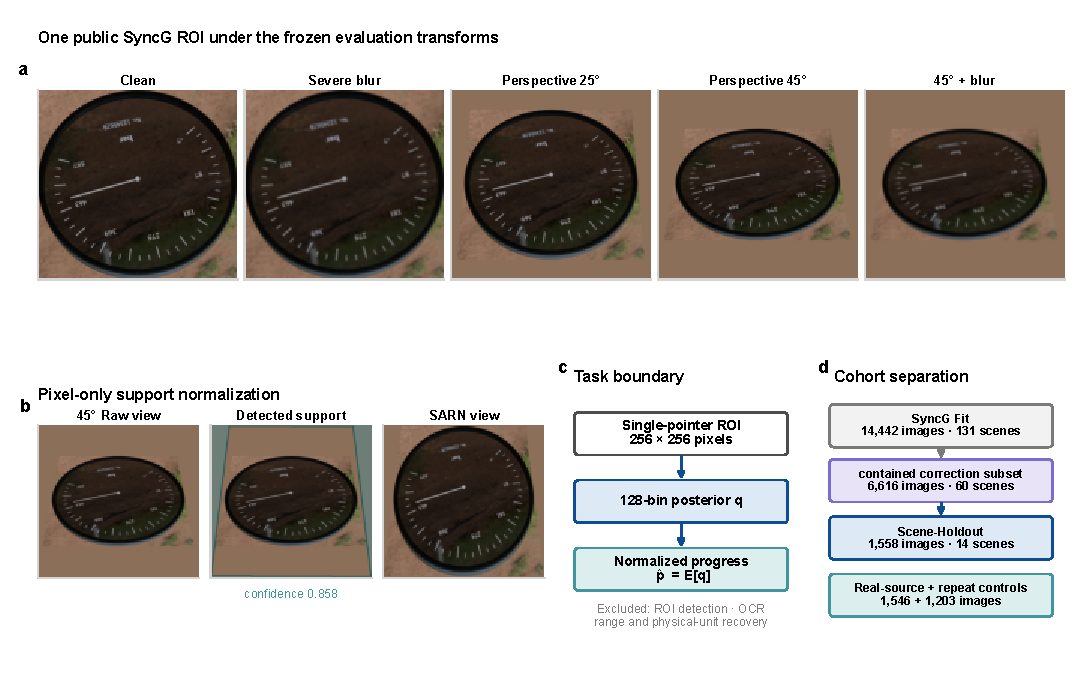
\includegraphics[width=\textwidth]{remstnet_task_scope.pdf}
\caption{Task, controlled observations, and evaluation separation. (\textbf{a}) One public SyncG single-pointer ROI under the clean, blur, and projective transforms used by the principal evaluation. The ROI was selected deterministically as a median projective-pool paired response among samples for which the relation was active in all three seeds; it illustrates the transforms and is not used as performance evidence. (\textbf{b}) The $45^{\circ}$ Raw view, detected pixel-only support, and resulting SARN view for the same ROI. (\textbf{c}) The core mapping from a $256\times256$ ROI to a 128-bin posterior and normalized progress; the separately evaluated field system boundaries prepend cached detection and, in Section~\ref{subsec:ocr_e2e_results}, existing OCR and automatic range recovery. (\textbf{d}) Dataset containment and group separation. The correction subset is contained within SyncG Fit, the Scene-Holdout scenes are disjoint from fitting, and all real/public-external and repeat cohorts are evaluation-only.}
\label{fig:task_scope}
\end{figure}

\subsection{Support-Aware Normalization and Paired Observations}
\label{subsec:sarn}

For an input ROI $I_r$, SARN-v2 constructs a second, pixel-derived observation $I_s$. It first tests whether flat and mutually consistent corner regions indicate full-canvas padding. Significant non-padding components are merged, their common convex hull is examined, and a frozen range of polygon approximation scales is searched for a reliable four-corner support. The principal fixed acceptance criteria include boundary-padding coverage of at least 0.90, support area between 0.30 and 0.84 of the canvas, quadrilateral-to-hull area ratio of at least 0.84, overall confidence of at least 0.72, and normalized crop area no greater than 0.92. When accepted, the support bounding box is cropped with a small margin and resized to the original canvas size. This operation supplies $I_s$, a valid-support mask $M$, and the exact crop--resize homography $H_{r\rightarrow s}$. It uses neither the target nor the known synthetic degradation transform.

If any support criterion fails, SARN-v2 is a bytewise no-op: $I_s=I_r$, $M=\mathbf{1}$, $H_{r\rightarrow s}=I_3$, and the relation-active indicator $a$ is zero. This conservative behavior is important for interpreting the clean and non-projective controls. SARN-v2 is designed to recognize its specific full-canvas projective-support pattern; it is not a general estimator of natural camera pose.

\subsection{Frozen Scalar Foundation and Moment-Matched Posterior Lifting}
\label{subsec:foundation}

The scalar foundation follows the EfficientNet-B0 stage widths \cite{tan2019efficientnet}: 40 channels at stride 8, 112 channels at stride 16, and a 1280-dimensional final representation. Its ImageNet-initialized point head was trained for 30 fixed epochs on SyncG Fit, using $256\times256$ inputs, batch size 64, Smooth-L1 loss with $\beta=0.05$, AdamW with learning rate $3\times10^{-4}$ and weight decay $10^{-4}$, and cosine annealing. The terminal iterate was used without selecting on Scene-Holdout. During subsequent \modelname\ training, the shared convolutional stages and scalar readout were frozen.

To expose a posterior interface without altering the frozen scalar mean $\mu$, the point prediction is lifted to a 128-bin distribution. A Gaussian-shaped base density with fixed scale $\sigma=0.025$ is formed on the progress grid,
\begin{equation}
b_k\propto\exp\left[-\frac{(x_k-\mu)^2}{2\sigma^2}\right],
\end{equation}
and is exponentially tilted to satisfy $\sum_kq_kx_k=\mu$. Twenty Newton updates solve the single natural parameter. The same construction is applied to the Raw and SARN views to obtain $\mathbf{q}_r$ and $\mathbf{q}_s$. Fixing $\sigma$ preserves a common transport geometry across runs but does not establish uncertainty calibration.

\subsection{Hierarchical Relation-Encoded Backbone}
\label{subsec:blocks}

Raw and SARN observations pass through the same frozen encoder. At feature strides $\ell\in\{8,16\}$, the SARN feature is differentiably aligned with the Raw feature by the crop homography, and the support mask is resized to the same scale. Let $P_{\ell}$ denote a learned projection to 48 relation channels, $U_r^{\ell}=P_{\ell}(F_r^{\ell})$, and $U_s^{\ell}=P_{\ell}(A_H(F_s^{\ell}))$. The relation tensor is
\begin{equation}
R_{\ell}=\left[
U_r^{\ell},U_s^{\ell},
U_s^{\ell}-U_r^{\ell},
\left|U_s^{\ell}-U_r^{\ell}\right|,
U_r^{\ell}\odot U_s^{\ell},
\cos(U_r^{\ell},U_s^{\ell}),
M^{\ell}
\right].
\label{eq:relation_tensor}
\end{equation}
Each ReMST block produces a 64-channel relation memory, a scalar local evidence value $e_{\ell}$, and a bounded feature residual,
\begin{equation}
\widetilde{F}_r^{\ell}=F_r^{\ell}
+0.1\,\tanh\!\left(C_{\ell}(R_{\ell})\right)\odot M^{\ell}.
\label{eq:feature_rewrite}
\end{equation}
The stride-8 residual is written back before stride-16 encoding, and the stride-16 residual is written back before context encoding. Hence later features depend on earlier Raw--SARN relations. Adaptive pooling maps each relation memory to a $4\times4$ grid, yielding 16 tokens per scale.

The relation is declared available only when SARN is active, the homography is finite and invertible for alignment, and both scale-specific support masks contain valid samples. The two blocks must both be available; partial availability does not trigger a correction.

\subsection{Progress-Aware Coordination and Adaptive Moment Budget}
\label{subsec:coordinator}

The cross-scale coordinator concatenates 16 tokens from each block, one explicit geometry token, and one context-change token, forming a 34-token memory. For each progress bin $k$, a nine-dimensional query is constructed:
\begin{equation}
z_k=\left[
q_{r,k},q_{s,k},\log q_{r,k},\log q_{s,k},
C_{r,k},C_{s,k},q_{s,k}-q_{r,k},
C_{s,k}-C_{r,k},x_k
\right],
\label{eq:bin_query}
\end{equation}
where $C_{r,k}$ and $C_{s,k}$ are cumulative probabilities. Two decoder layers with four attention heads map the 128 bin queries into 64-dimensional progress tokens. Within each layer, a depthwise one-dimensional convolution of kernel size 5, followed by GELU and pointwise mixing, exchanges evidence among neighboring bins. This local progress mixing is intentionally narrower than unrestricted all-bin self-attention.

The decoder yields progress evidence $e_p$; the two blocks and the context path yield $e_8$, $e_{16}$, and $e_c$. One global learned scalar $\rho$ sets a bounded budget gain, while the evidence remains sample-specific:
\begin{align}
g &= 1+0.5\tanh(\rho), \qquad 0.5<g<1.5, \\
\Delta &= 0.025\,g\,\tanh\left(
e_p+\frac{\tanh(e_8)+\tanh(e_{16})+\tanh(e_c)}{3}
\right), \label{eq:total_shift}\\
\boldsymbol{\alpha} &=
\operatorname{softmax}\!\left[
\tanh(e_8),\tanh(e_{16}),\tanh(e_c)
\right], \\
\delta_j&=\alpha_j\Delta,\qquad j\in\{8,16,c\}.
\label{eq:allocation}
\end{align}
Thus $\alpha_j\geq0$, $\sum_j\alpha_j=1$, and all three requested stage shifts have the sign of $\Delta$. Their sum is exactly the bounded requested displacement, so the stages cannot request opposing corrections. The zero initialization gives $\Delta=0$ and reproduces the SARN endpoint on relation-valid samples.

\subsection{Moment-Exact Information Projection and Fallback}
\label{subsec:transport}

Starting from $\mathbf{q}^{(0)}=\mathbf{q}_s$, the feasible target for stage $j$ is
\begin{equation}
t_j=\operatorname{clip}_{[\varepsilon_{32},\,1-\varepsilon_{32}]}
\left(\mathbb{E}_{\mathbf{q}^{(j)}}[x]+\delta_j\right),
\label{eq:feasible_target}
\end{equation}
where $\varepsilon_{32}$ is the positive FP32 machine epsilon used by the implementation. Each stage then computes the information projection
\begin{equation}
\mathbf{q}^{(j+1)}
=\arg\min_{\mathbf{q}\in\Delta^{K-1}}
D_{\mathrm{KL}}\!\left(\mathbf{q}\,\|\,\mathbf{q}^{(j)}\right)
\quad\mathrm{s.t.}\quad
\mathbb{E}_{\mathbf{q}}[x]
=t_j.
\label{eq:iprojection}
\end{equation}
The discrete solution has the exponential-tilt form \cite{csiszar1975idivergence}
\begin{equation}
q_k^{(j+1)}
=\frac{q_k^{(j)}\exp(\lambda_jx_k)}
{\sum_mq_m^{(j)}\exp(\lambda_jx_m)},
\label{eq:exponential_tilt}
\end{equation}
where $\lambda_j$ is solved with 20 Newton iterations. The solver is evaluated in FP32, and the implementation tests require the observed first moment to match $t_j$ within $2\times10^{-6}$. In this paper, ``moment-exact'' denotes this feasible-target equality to numerical tolerance, not symbolic exact arithmetic. If every requested intermediate target is feasible without clipping, the terminal mean equals $\mathbb{E}_{\mathbf{q}_s}[x]+\Delta$. Near 0 or 1, clipping can shorten the realized displacement, but each stage remains non-opposing by construction up to solver tolerance. The decomposition connects the requested mean change to hierarchical evidence and supplies inspectable intermediate posteriors rather than enlarging the scalar function class through repeated projection.

If the Raw--SARN relation is unavailable, Equation~\eqref{eq:iprojection} is not evaluated as a learned alternative and the network returns $\mathbf{q}^{*}=\mathbf{q}_r$ exactly. If it is available but $\Delta=0$, the terminal posterior equals $\mathbf{q}_s$ exactly. The fallback is controlled only by whether the geometric relation is defined. It does not inspect target values, compare expert errors, or use a learned confidence router.

Figure~\ref{fig:architecture} summarizes the evidence path, feasible moment transport, and the two exact fallback identities.

\begin{figure}[H]
\centering
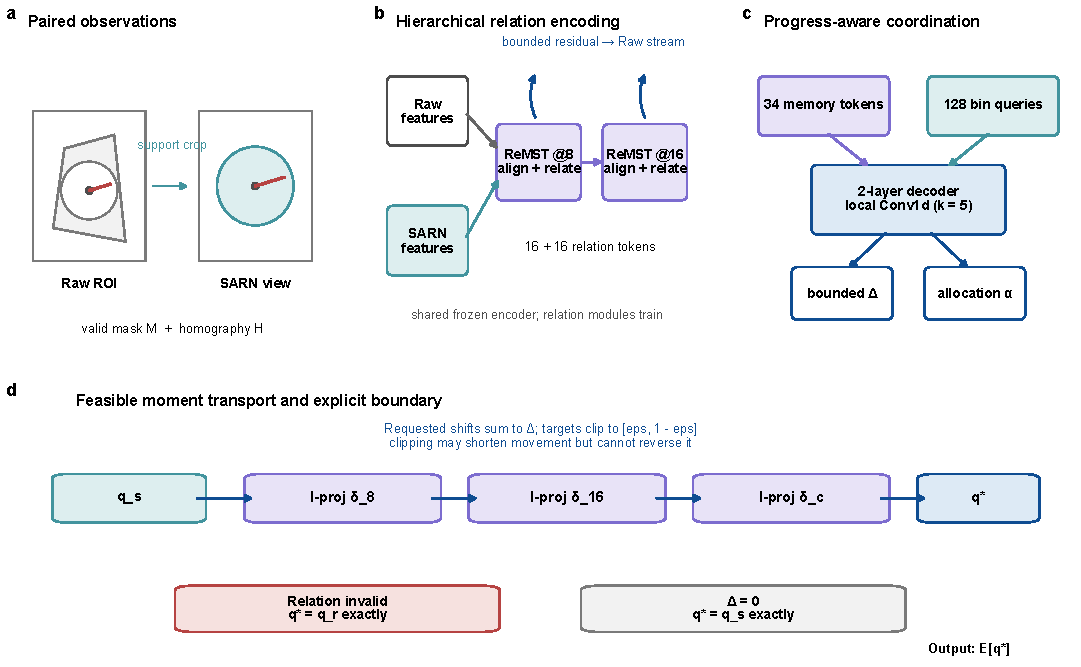
\includegraphics[width=\textwidth]{remstnet_architecture.pdf}
\caption{\modelname\ architecture and boundary behavior. (\textbf{a}) The model receives the Raw ROI and the support-aware normalized SARN view with its mask and crop homography. (\textbf{b}) Shared frozen features are aligned and related at strides 8 and 16; bounded residuals rewrite the Raw stream. (\textbf{c}) A 34-token relation memory conditions 128 progress-bin queries, and the coordinator predicts a bounded displacement $\Delta$ and non-negative allocation $\boldsymbol{\alpha}$. (\textbf{d}) Three information projections match feasible clipped moment targets. Requested shifts sum to $\Delta$ and share its sign, although boundary clipping may shorten realized movement. Undefined geometry returns the Raw posterior exactly, whereas $\Delta=0$ returns the SARN endpoint exactly.}
\label{fig:architecture}
\end{figure}

\subsection{Training Objective and Reproducibility}
\label{subsec:training}

Each correction-training image produced a synchronized triplet at $25^{\circ}$ perspective, $45^{\circ}$ perspective, and $45^{\circ}$ perspective plus severe blur. A physical batch contained eight source images and therefore 24 condition rows. Only the 261,528 parameters of the two ReMST blocks and coordinator were optimized; the 4,010,110 foundation parameters remained frozen and were compared tensor-by-tensor before and after training.

For a relation-active row, $\mathcal{L}_{\mathrm{read}}$ averages normalized two-hot posterior cross-entropy and normalized Smooth-L1 mean error. $\mathcal{L}_{\mathrm{path}}$ compares the CDFs of eight natural-geodesic intermediate posteriors with a linear CDF path from the Raw anchor to the target. $\mathcal{L}_{\mathrm{excess}}$ is a one-sided hinge on the amount by which final absolute error exceeds the detached SARN-endpoint error. $\mathcal{L}_{\mathrm{CVaR}}$ is the mean absolute error in the worst 25\% of active rows, $\mathcal{L}_{W_1}$ is the mean pairwise one-dimensional Wasserstein discrepancy among the three synchronized condition posteriors of one physical sample, and $\mathcal{L}_{\mathrm{energy}}$ penalizes squared displacement. Error and CDF regularizers were normalized by 0.05. The total loss was
\begin{equation}
\mathcal{L}=
\mathcal{L}_{\mathrm{read}}
+0.10\mathcal{L}_{\mathrm{path}}
+\mathcal{L}_{\mathrm{excess}}
+0.25\mathcal{L}_{\mathrm{CVaR}}
+0.05\mathcal{L}_{W_1}
+10^{-4}\mathcal{L}_{\mathrm{energy}}.
\label{eq:loss}
\end{equation}

Three ReMST fits were initialized from the seed-matched terminal EfficientNet-B0 foundations with source seeds 20262020, 20262021, and 20262022. Their ReMST initialization seeds were 20262213--20262215 and their sample-order seeds were 20262217--20262219. Each fit used exactly five terminal epochs, AdamW with learning rate $3\times10^{-4}$ and weight decay $10^{-4}$, a five-epoch cosine schedule, and BF16 autocast on the RTX 4060; posterior construction and feasible moment transport were evaluated in FP32.

\subsection{Baselines, Metrics, and Statistical Analysis}
\label{subsec:evaluation}

The baselines followed a matched training protocol: SARN-v2 was paired with Direct-ResNet18 \cite{he2016resnet}, EfficientNet-B0 \cite{tan2019efficientnet}, or MobileNetV3-Large \cite{howard2019mobilenetv3}. Direct-ResNet18 denotes a ResNet18 encoder with a direct scalar progress head rather than a detection or segmentation pipeline. Each baseline was ImageNet-initialized and trained on the same 14,442-image SyncG Fit roster for 30 fixed epochs with the same input size, scalar loss, optimizer, schedule, augmentation contract, and three source seeds. The seed-matched SARN-v2+EfficientNet-B0 prediction is also the endpoint from which each \modelname\ model was initialized, enabling a direct estimate of the additional relation-transport contribution.

VDN was added as a secondary external-architecture comparator rather than as a row in the primary table \cite{dong2021vdn}. The evaluated checkpoint was one local terminal epoch-200 run of the upstream VDN architecture retrained on 14,375 SyncG images; it was not an official pretrained weight. Its independently fixed 1,625-image grouped holdout differed from the 1,558-image ReMSTNet Scene-Holdout. We selected their prediction-independent intersection: 129 samples from six ReMSTNet scene stems, with the same complete six-condition pixel set (774 rows), and verified pixel identities before scoring. For VDN only, the annotated pivot and ordered scale endpoints were used to convert its predicted direction into normalized progress on every row. ReMSTNet and EfficientNet-B0 predicted progress directly without those annotations. Neither automatic-reference success nor automatic-reference error was used to select rows for the paper-facing comparison; that branch was retained only as an implementation diagnostic. This provides a full-coverage direction-component comparison, not an input-equivalent deployable-system comparison.

The organized industrial ROI baseline and two diagnostic tracks were added without fitting or adaptation. The industrial baseline pools the exact 1,395-ROI union described above and applies the same clean, two blur, and three controlled projective conditions. RPM-10K uses the 1,797-image scalar-reading subset and existing detector-produced crops; detector or reader failure receives normalized error 1 on the full denominator. Its evaluator deliberately supplies identical raw and normalized images, unit support, an inactive relation mask, and identity homography, so it measures only the frozen raw foundation inside the ReMST wrapper and cannot test relation gains. The Industrial Full-Frame Diagnostic uses existing best-confidence YOLO boxes for all 153 deduplicated deployment photographs, including 33 scalar-labeled frames. Unlabeled frames contribute only to detector/read coverage, and the absence of bounding-box ground truth prevents detector recall or IoU estimation.

The end-to-end physical-reading replay was executed as a separate prediction-then-scoring experiment on the same 153 photographs. Its label-free prediction pass read only the raw-photo inventory and cached detector boxes, reran all three ReMSTNet checkpoints, and combined normalized progress with the existing PP-OCRv4 mobile recognizer and production start/end-point geometry. PP-OCRv4 belongs to the lightweight PP-OCR family \cite{du2020ppocr}; local inference used RapidOCR with ONNX Runtime \cite{rapidocr2026}. The OCR weights were used unchanged. The decoder default confidence of 0.55 is the primary operating point, while 0.95 is reported only as a transferred sensitivity because the field replay uses the available production point geometry. No decoder threshold or range rule was fitted to the field photographs.

For a labeled physical reading $y_i$ with ordered true range $[a_i,b_i]$, physical-unit normalized absolute error was $|\hat{y}_i-y_i|/|b_i-a_i|$. Conditional NMAE averages this quantity only over accepted range outputs. Full-denominator NMAE retains every labeled photograph, assigns error 1 to missing stage output, and leaves finite wrong readings uncapped; the bounded counterpart clips finite errors at 1. The same accepted subset was also rescored with the true range while preserving each ReMSTNet progress estimate, providing a matched oracle-range comparator for the incremental range-stage error. Accuracy uses only the 33 labeled photographs, whereas coverage uses all 153.

The primary metric was full-denominator normalized mean absolute error,
\begin{equation}
\mathrm{NMAE}=\frac{1}{N}\sum_{i=1}^{N}|\hat{p}_i-p_i|.
\end{equation}
Because the target is already normalized, this is also MAE in full-scale units. A missing or non-finite prediction, had one occurred, was assigned error 1; coverage reports the fraction of finite predictions. Accuracy at tolerance $\tau$ was $\mathrm{Acc}@\tau=N^{-1}\sum_i\mathbb{1}(|\hat{p}_i-p_i|\leq\tau)$. RMSE and tail percentiles were retained as secondary diagnostics.

Tables report the mean and sample standard deviation across three independently trained models, not a prediction ensemble. For paired inference, the absolute error of each row was first averaged across the three seeds; complete scene or source groups were then resampled 20,000 times with replacement, and percentile 95\% confidence intervals were computed for $\Delta\mathrm{NMAE}=\mathrm{NMAE}_{\modelname}-\mathrm{NMAE}_{\mathrm{comparator}}$ \cite{davison1997bootstrap}. These intervals quantify observed-group sampling variation after seed averaging; they do not estimate the full distribution of outcomes from retraining. The factorial ablation used one fixed source seed, so its paired scene-bootstrap intervals capture group sampling only and exclude training-seed uncertainty. Intervals are dataset-wise, estimation-focused, and unadjusted for multiple comparisons.

For the VDN intersection, ReMSTNet and EfficientNet-B0 errors were averaged row-wise across their three fitted seeds on all 774 rows before paired resampling of the six ReMSTNet scene groups. VDN had one terminal checkpoint, so these intervals include neither VDN retraining uncertainty nor a common training-roster comparison. Because VDN receives annotation-derived reference geometry for offline conversion, the comparison isolates direction-component quality and is not a system-wide automatic-reader comparison.

An additional single-seed stress sweep used 18 conditions: clean; perspective at 15, 30, 45, and $60^{\circ}$; sensor-noise standard deviations 0.01, 0.03, and 0.05 on the $[0,1]$ scale; brightness factors 0.60, 0.80, 1.20, and 1.40; JPEG quality 80, 50, and 20; and nested, deterministically placed occlusions covering 5\%, 10\%, and 20\% of the image. Finally, CUDA efficiency was measured in independent processes on an NVIDIA GeForce RTX 4060 with PyTorch 2.11.0, CUDA 12.8, and BF16. Eight fixed severe-perspective images were profiled at batch sizes 1 and 8 using 20 warm-up and 100 timed iterations. Timings included pinned host-to-device transfer, all model forwards, posterior checks, and synchronization, but excluded image decoding, checkpoint loading, and SARN image materialization.

\subsection{Generative AI Assistance}

During preparation of this manuscript, the authors used OpenAI Codex [product version and access date to be completed by the authors] to assist with manuscript drafting, generation of figure source code, and consistency checks among the manuscript, source code, and stored aggregate result files. The underlying experimental data and model checkpoints predated this manuscript-preparation pass; Codex did not retrain the models or create the reported measurements. The authors reviewed and edited the generated material and remain responsible for the study design, analyses, interpretations, citations, and final text. The authors must verify this statement against any broader use of generative AI before submission.

\section{Results}
\label{sec:results}

\subsection{Scene-Disjoint SyncG Comparison}
\label{subsec:syncg_results}

All four methods produced finite outputs for every row. Because this fixed scene-disjoint roster has supported repeated method comparisons, the estimates below are retrospective same-domain benchmark results rather than untouched confirmation. Table~\ref{tab:main_results} shows that the advantage of \modelname\ was concentrated in projective conditions. Direct-ResNet18 had the smallest point estimate for clean and both blur conditions, while \modelname\ and its EfficientNet-B0 endpoint were numerically equivalent at the displayed precision in these no-relation cases. At $25^{\circ}$, $45^{\circ}$, and $45^{\circ}$ plus blur, \modelname\ reduced NMAE relative to every comparator.

\begin{table}[H]
\caption{SyncG Scene-Holdout NMAE across three independent training seeds (mean $\pm$ sample SD). The Proj. column pools the three projective conditions. The lowest value in each column is bold.}
\label{tab:main_results}
\centering
\resizebox{\textwidth}{!}{%
\begin{tabular}{lcccccccc}
\toprule
\textbf{Method} & \textbf{Clean} & \textbf{Blur-M} & \textbf{Blur-S} & \textbf{Persp.-25} & \textbf{Persp.-45} & \textbf{45+Blur} & \textbf{All} & \textbf{Proj.} \\
\midrule
SARN-v2 + Direct-ResNet18
& $\mathbf{0.007910\pm0.000411}$ & $\mathbf{0.007932\pm0.000397}$ & $\mathbf{0.008207\pm0.000420}$
& $0.014422\pm0.000343$ & $0.024302\pm0.000398$ & $0.026219\pm0.000564$
& $0.014832\pm0.000346$ & $0.021648\pm0.000435$ \\
SARN-v2 + EfficientNet-B0
& $0.008099\pm0.000323$ & $0.008064\pm0.000338$ & $0.008282\pm0.000472$
& $0.014177\pm0.000607$ & $0.021578\pm0.000968$ & $0.023411\pm0.000995$
& $0.013935\pm0.000606$ & $0.019722\pm0.000852$ \\
SARN-v2 + MobileNetV3-Large
& $0.009355\pm0.000435$ & $0.009421\pm0.000489$ & $0.009807\pm0.000385$
& $0.016255\pm0.000489$ & $0.025584\pm0.001962$ & $0.027589\pm0.001664$
& $0.016335\pm0.000716$ & $0.023143\pm0.001361$ \\
\textbf{\modelname-v3}
& $0.008099\pm0.000323$ & $0.008064\pm0.000338$ & $0.008282\pm0.000471$
& $\mathbf{0.010330\pm0.000476}$ & $\mathbf{0.013884\pm0.000441}$ & $\mathbf{0.015564\pm0.000299}$
& $\mathbf{0.010704\pm0.000373}$ & $\mathbf{0.013259\pm0.000391}$ \\
\bottomrule
\end{tabular}}
\end{table}

Across all six conditions, the relative NMAE reductions versus Direct-ResNet18, EfficientNet-B0, and MobileNetV3-Large were 27.83\%, 23.19\%, and 34.47\%, respectively. For the projective pool, the corresponding reductions were 38.75\%, 32.77\%, and 42.71\%. The all-condition paired $\Delta$NMAE confidence intervals were
\[
\begin{aligned}
\text{Direct-ResNet18:}\quad &[-0.004604,-0.003665],\\
\text{EfficientNet-B0:}\quad &[-0.003522,-0.002896],\\
\text{MobileNetV3-Large:}\quad &[-0.006455,-0.004768].
\end{aligned}
\]
All three intervals were below zero. These aggregate results should be read together with the clean/blur columns: \modelname\ improved the conditions for which its geometric relation was active, rather than uniformly improving every input.

Figure~\ref{fig:core_performance} complements the aggregate table with row-, scene-, and target-level views of the comparison with the seed-matched EfficientNet-B0 endpoint. The decompositions show that the projective gain was not produced by a single scene or a narrow target interval, while also exposing the minority of rows for which transport increased absolute error.

\begin{figure}[H]
\centering
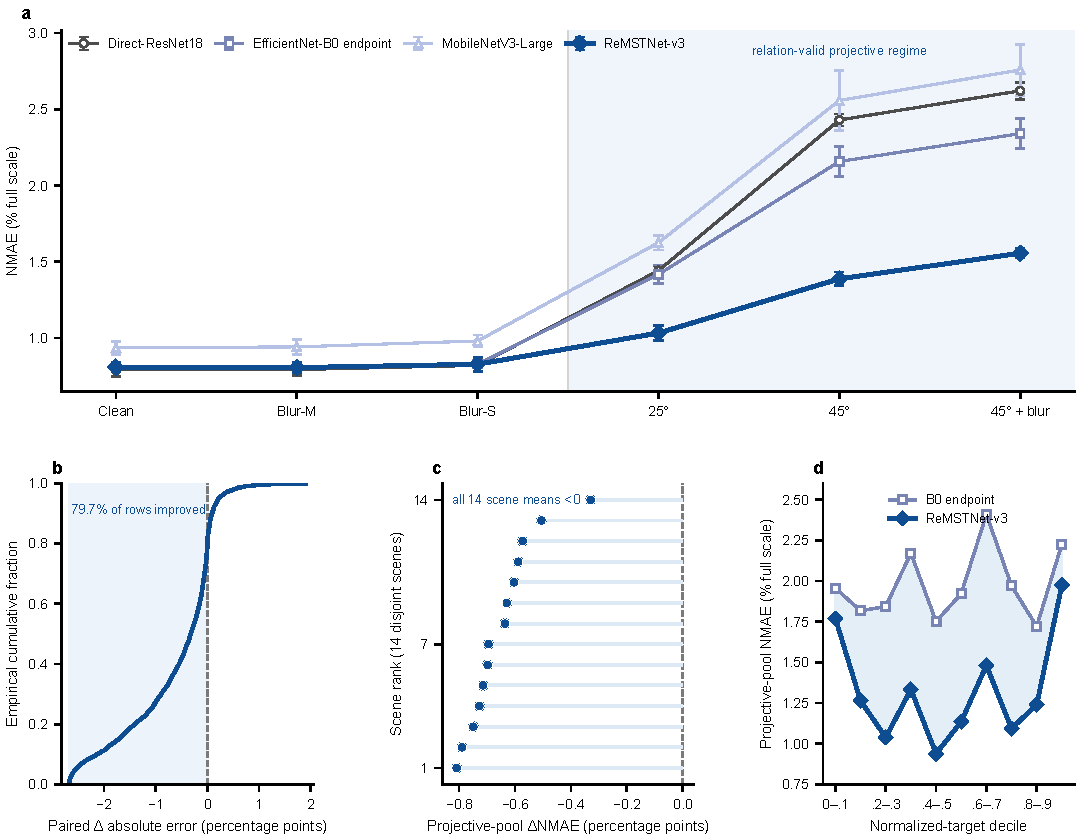
\includegraphics[width=\textwidth]{remstnet_core_performance.pdf}
\caption{Core same-domain performance at complementary aggregation levels. (\textbf{a}) Condition-wise NMAE; points and error bars are the mean and sample SD across three independently trained models, and the shaded region marks the relation-valid projective regime. (\textbf{b}) Empirical cumulative distribution of the paired projective-row change in absolute error for \modelname\ minus the seed-matched SARN-v2+EfficientNet-B0 endpoint. Absolute errors were first averaged row-wise across the three seeds ($4674$ rows); negative values favor \modelname. (\textbf{c}) Projective-pool paired $\Delta$NMAE for each of the 14 scene-disjoint groups. (\textbf{d}) Projective-pool NMAE across normalized-target deciles for the endpoint and \modelname. Panels (\textbf{b})--(\textbf{d}) are descriptive decompositions of the registered comparison rather than additional multiplicity-adjusted inferential tests.}
\label{fig:core_performance}
\end{figure}

\subsection{Secondary VDN Annotation-Assisted Comparison}
\label{subsec:vdn_results}

The two pre-existing holdouts overlapped on 129 samples from six ReMSTNet scene groups, producing 774 fixed same-pixel condition rows. Table~\ref{tab:vdn_intersection} uses every row. Its reported coverage is therefore 774/774 for all conditions and 387/387 for the projective pool, rather than a denominator conditioned on VDN success. For VDN, annotation-derived pivot and ordered scale endpoints convert its direction prediction into progress; the two scalar readers do not receive this information. Consequently, the table measures the VDN direction component against direct progress readers at full coverage rather than the deployability of VDN's automatic reference stage.

\begin{table}[H]
\caption{Secondary annotation-assisted VDN same-pixel comparison inside the fixed 129-sample holdout intersection. ReMSTNet and B0 values are mean $\pm$ sample SD across three fits; VDN uses one terminal epoch-200 checkpoint. VDN's annotated pivot and ordered scale endpoints are used only for offline direction-to-progress conversion. The paired difference is ReMSTNet minus VDN after row-wise seed averaging.}
\label{tab:vdn_intersection}
\centering
\resizebox{\textwidth}{!}{%
\begin{tabular}{lrrrrr}
\toprule
\textbf{Scope} & \textbf{Rows / Fixed} & \textbf{Coverage} & \textbf{\modelname-v3 NMAE} & \textbf{B0 NMAE} & \textbf{VDN NMAE / $\Delta$ (95\% CI)} \\
\midrule
All conditions & 774 / 774 & 100\% & $\mathbf{0.008582\pm0.000414}$ & $0.011673\pm0.000638$ & $0.016444$ / $-0.007861$ $[-0.012340,-0.005530]$ \\
Projective pooled & 387 / 387 & 100\% & $\mathbf{0.010938\pm0.000935}$ & $0.017119\pm0.001396$ & $0.021030$ / $-0.010092$ $[-0.014298,-0.006818]$ \\
\bottomrule
\end{tabular}}
\end{table}

Across all rows and the projective pool, \modelname\ reduces NMAE relative to the annotation-assisted VDN reference by 47.81\% and 47.99\%, respectively, and both paired intervals are below zero. The comparison nevertheless contains only six scene clusters, omits VDN retraining uncertainty, and supplies VDN with annotated reference geometry. It is therefore strong supporting evidence for the learned pointer representation on identical pixels, but not a deployable-system ranking or a replacement for the primary matched-roster comparison.

\subsection{Public External and Industrial Full-Frame Diagnostics}
\label{subsec:external_native_results}

Table~\ref{tab:external_native} retains a public raw-foundation cross-domain diagnostic and directly exercises the organized deployment photographs. RPM-10K supplies scalar readings and ordered ranges but no relation input under the released single-view protocol. The full-frame track begins from the original industrial scene photograph rather than a prepared ROI.

\begin{table}[H]
\caption{Public raw-foundation and industrial full-frame diagnostics. Mean $\pm$ sample SD is across three fits. Full-frame coverage uses all 153 photographs, whereas its NMAE uses the 33 scalar-labeled frames.}
\label{tab:external_native}
\centering
\resizebox{\textwidth}{!}{%
\begin{tabular}{lllll}
\toprule
\textbf{Track} & \textbf{Task / Method} & \textbf{Metric denominator} & \textbf{Detection/read coverage} & \textbf{Primary metric} \\
\midrule
RPM-10K single-pointer & scalar / \modelname-v3 & 1,797 labeled images & 1,775/1,797 (98.78\%) & NMAE $0.233945\pm0.012331$ \\
Industrial Full-Frame & scalar / cached detector + \modelname-v3 & 33 labeled; 153 coverage frames & 151/153 (98.69\%) & NMAE $0.051930\pm0.001031$ \\
\bottomrule
\end{tabular}}
\end{table}

On RPM-10K, 22 detector failures were assigned error 1 on the full 1,797-image denominator. Acc@2\% was $10.55\pm2.01$\%, Acc@5\% was $24.43\pm1.04$\%, and the row-wise three-seed mean NMAE had a stratified image-bootstrap 95\% CI of $[0.225546,0.242634]$. The subset is not degradation-free: 474 images carry a blur tag, 993 a tilted-view tag, and 157 both. Nevertheless, the evaluator supplies identical raw/normalized images, unit support, an inactive relation mask, and identity homography. Equality with B0 is therefore imposed by the protocol; the number diagnoses raw-foundation transfer and is not evidence for or against relation-module benefit on RPM-10K.

The full-frame diagnostic uses 153 unique photographs from the repository's industrial \texttt{data/} and \texttt{data-717/} directories, deduplicated into the organized deployment roster. Existing best-confidence YOLO boxes produced readings for 151 frames; two returned \texttt{meter\_not\_found}. All 33 labeled frames passed and yielded Acc@2\% of $34.34\pm13.66$\%, Acc@5\% of $70.71\pm1.75$\%, and a row-wise mean NMAE bootstrap 95\% CI of $[0.032544,0.079142]$. The other 120 photographs contribute to coverage only. This first replay is a retrospective cached-detector scalar-reader diagnostic rather than a detector benchmark, because no box ground truth is available; OCR and automatic physical-range recovery are evaluated separately below.


\subsection{Independent End-to-End Physical-Reading Deployment Replay}
\label{subsec:ocr_e2e_results}

The independent deployment replay evaluates the complete full-photo-to-physical-reading chain: cached meter detection, three ReMSTNet progress estimates, unchanged PP-OCRv4 and point geometry, automatic range decoding, and physical-unit conversion. Across all 153 deployment photographs, cached boxes existed for 151, at least one numeric OCR token was recovered for 83, the default decoder produced 27 physical readings (17.65\%), and the transferred 0.95 sensitivity produced five (3.27\%). Table~\ref{tab:ocr_e2e} separates this coverage from accuracy on the 33 labeled photographs. The default decoder accepted nine labeled photographs. Their conditional physical-unit NMAE was $0.036814\pm0.004015$, while the same ReMSTNet predictions evaluated with the true ranges on exactly those nine photographs gave $0.034336\pm0.003848$. The matched incremental range-stage difference was therefore $+0.002478\pm0.002546$ NMAE. Conditional Acc@5\% was $70.37\pm6.42$\%. Six of nine recovered range pairs placed both endpoints within 5\% of the true span, and all nine were within 10\%.

\begin{table}[H]
\caption{End-to-end physical-reading results with existing OCR. Mean $\pm$ sample SD is across the three ReMSTNet fits. Conditional and matched-oracle columns use the identical accepted photographs within each row. Full-denominator NMAE assigns error 1 to a missing output on any of the 33 labeled photographs.}
\label{tab:ocr_e2e}
\centering
\resizebox{\textwidth}{!}{%
\begin{tabular}{lccccc}
\toprule
\textbf{Operating point} & \textbf{All-photo outputs} & \textbf{Labeled outputs} & \textbf{Conditional NMAE} & \textbf{Matched oracle-range NMAE} & \textbf{Full-denominator NMAE} \\
\midrule
Decoder default (0.55) & 27/153 (17.65\%) & 9/33 (27.27\%) & $0.036814\pm0.004015$ & $0.034336\pm0.003848$ & $0.737313\pm0.001095$ \\
Transferred 0.95 sensitivity & 5/153 (3.27\%) & 2/33 (6.06\%) & $0.037650\pm0.004240$ & $0.016195\pm0.007200$ & $0.941676\pm0.000257$ \\
\bottomrule
\end{tabular}}
\end{table}

\begin{figure}[H]
\centering
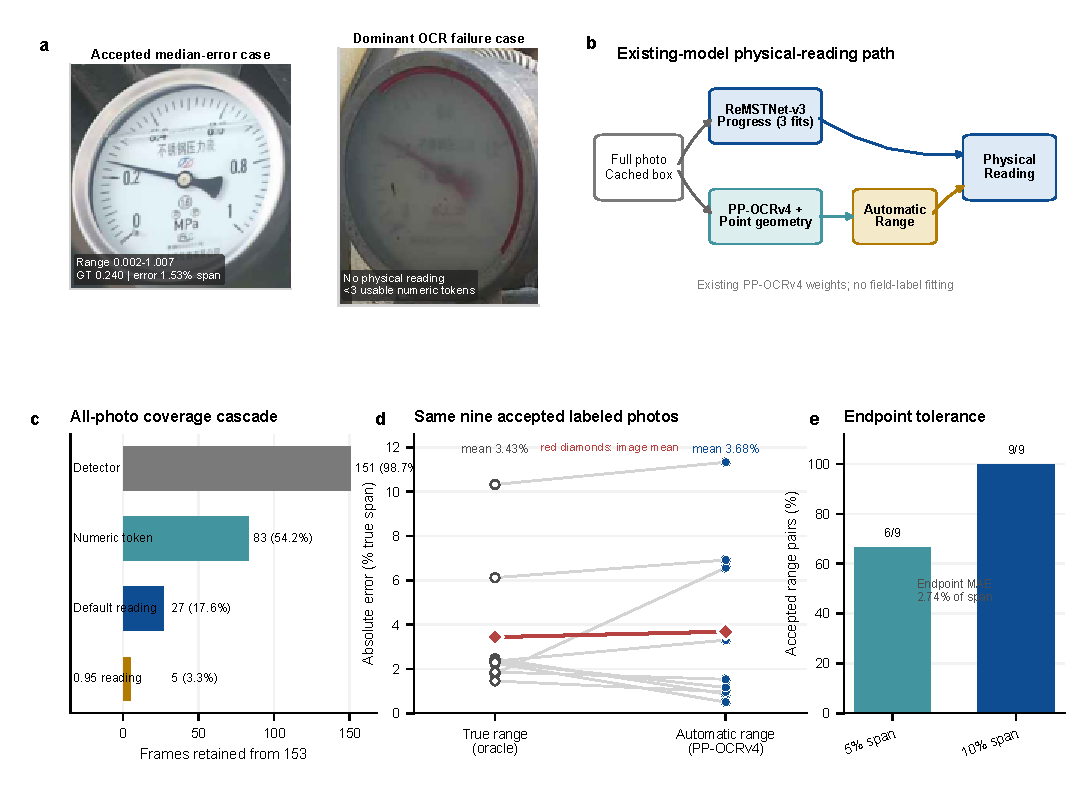
\includegraphics[width=\textwidth]{remstnet_ocr_end_to_end_deployment.pdf}
\caption{End-to-end physical-reading deployment replay with existing OCR. (\textbf{a}) Unadjusted detector crops show the median automatic-range error among the nine accepted labeled photographs and the median sample identifier within the most frequent labeled decoder-failure category; selection rules were deterministic and the examples are illustrative. (\textbf{b}) The path combines cached detection, three ReMSTNet progress estimates, unchanged PP-OCRv4, existing point geometry, automatic range decoding, and physical-unit conversion; no field label was used for OCR or threshold fitting. (\textbf{c}) Coverage cascade over all 153 photographs. The 0.95 row is a transferred sensitivity, not the primary operating point. (\textbf{d}) Paired row-wise three-fit mean absolute errors on the identical nine default-accepted labeled photographs under true versus automatic ranges; red diamonds show the image means. (\textbf{e}) Fraction of those nine range pairs whose two endpoints fall within 5\% or 10\% of the true span. Accuracy uses $n=33$ labeled photographs, coverage uses $n=153$, and no hypothesis test was applied. Source data are provided as CSV files with the figure.}
\label{fig:ocr_e2e}
\end{figure}

The favorable conditional error does not imply full-pipeline coverage: assigning error 1 to each missing labeled output raises default full-denominator NMAE to $0.737313\pm0.001095$. The dominant all-photo diagnostic was fewer than three usable numeric tokens (97 frames); diagnostic categories can overlap across operating points. The stricter 0.95 threshold retained only 2/33 labeled photographs and is therefore not a practical primary setting. On the local workstation, OCR alone required 65.68~s for 153 photographs, OCR plus range decoding 77.84~s, and the three ReMSTNet passes 15.56~s. Cached boxes exclude live detector time, so these are stage totals rather than acquisition-to-result latency. A complete independent rerun reproduced every per-image prediction and metric apart from runtime. The experiment therefore establishes that existing OCR can preserve the reader's accuracy on accepted photographs, while text and range-output coverage remains the immediate deployment bottleneck.

\subsection{Frozen Real-Source Cohort Evaluation}
\label{subsec:real_results}

Table~\ref{tab:real_results} reports the unified industrial baseline, its three source subdivisions, and RF100-derived. The source images were evaluated clean and under the same five controlled degradations; no real-domain fitting or model choice was performed. The bold parent row pools the exact 1,395-ROI industrial denominator and does not add images to its three subdivisions.

\begin{table}[H]
\caption{Frozen six-condition real-source cohort NMAE (mean $\pm$ sample SD across seeds) and paired group-bootstrap differences computed after row-wise averaging across the three seeds. Negative $\Delta$ favors \modelname.}
\label{tab:real_results}
\centering
\resizebox{\textwidth}{!}{%
\begin{tabular}{lrrcccc}
\toprule
\textbf{Cohort} & \textbf{Images} & \textbf{Groups} & \textbf{\modelname-v3} & \textbf{SARN-v2+B0} & \textbf{$\Delta$NMAE} & \textbf{95\% CI} \\
\midrule
\textbf{Industrial Real-Photo Baseline} & \textbf{1,395} & \textbf{52} & $\mathbf{0.123388\pm0.018553}$ & $0.123664\pm0.018317$ & $\mathbf{-0.000276}$ & $\mathbf{[-0.000382,-0.000168]}$ \\
FieldGauge-ROI Test-A & 434 & 11 & $0.116689\pm0.012464$ & $0.116963\pm0.012283$ & $-0.000275$ & $[-0.000438,-0.000116]$ \\
FieldGauge-ROI Test-B & 814 & 20 & $0.112915\pm0.015050$ & $0.113247\pm0.014806$ & $-0.000332$ & $[-0.000487,-0.000177]$ \\
FieldGauge-External-ROI & 147 & 21 & $0.201162\pm0.057755$ & $0.201135\pm0.057342$ & $+0.000027$ & $[-0.000106,+0.000155]$ \\
RF100-derived cohort & 151 & 35 & $0.050289\pm0.015948$ & $0.051548\pm0.015739$ & $-0.001259$ & $[-0.001893,-0.000530]$ \\
\bottomrule
\end{tabular}}
\end{table}

Within the industrial baseline, the projective pool was $0.122590\pm0.015220$ for \modelname\ and $0.123142\pm0.014802$ for B0, with paired $\Delta=-0.000552$ and 95\% CI $[-0.000761,-0.000335]$. Each individual projective condition also favored \modelname. Moderate perspective gave $\Delta=-0.000316$ (95\% CI $[-0.000513,-0.000090]$), severe perspective gave $\Delta=-0.000632$ ($[-0.000859,-0.000404]$), and severe perspective plus blur gave $\Delta=-0.000709$ ($[-0.001011,-0.000420]$). Thus, the relation gain transfers consistently to controlled projective variants of industrial photographs, although its absolute magnitude is smaller than on SyncG.

On native clean and blur-only rows, \modelname\ and the endpoint were numerically equivalent because the defined projective-support relation was inactive. The result therefore does not demonstrate automatic correction of arbitrary as-captured obliquity or generic blur. FieldGauge-External-ROI alone remains unresolved at its present group resolution, but its smaller 147-image weight does not erase the paired effect on the predeclared 1,395-image pooled industrial denominator.

Figure~\ref{fig:real_transfer} separates the real-source result into cohort aggregates, controlled conditions, and source-group effects. This view preserves the unresolved External-ROI comparison and the near-zero clean/blur effects instead of allowing the favorable RF100-derived projective effect to dominate the visual summary.

\begin{figure}[H]
\centering
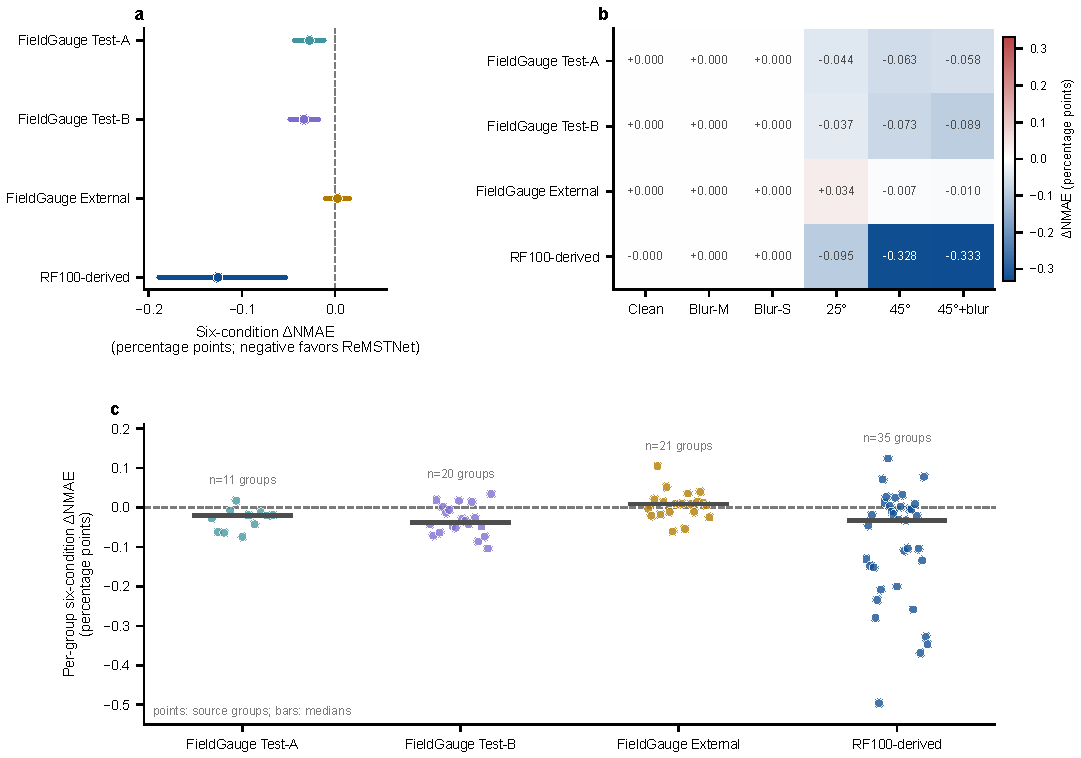
\includegraphics[width=\textwidth]{remstnet_real_transfer.pdf}
\caption{Frozen real-source transfer relative to the seed-matched SARN-v2+EfficientNet-B0 endpoint. (\textbf{a}) Six-condition cohort $\Delta$NMAE and 95\% group-bootstrap intervals after absolute errors were averaged row-wise across three seeds. (\textbf{b}) Condition-by-cohort $\Delta$NMAE in percentage points; the clean and blur-only cells are zero at displayed precision because the projective-support relation was inactive. (\textbf{c}) The corresponding effects for all 87 source groups, with horizontal bars denoting cohort medians. Negative values favor \modelname. FieldGauge images are subject to project permissions and are therefore not displayed; no real-source image or label was used for fitting or model selection.}
\label{fig:real_transfer}
\end{figure}

\subsection{Factorial Mechanism Analysis}
\label{subsec:ablation_results}

The $2\times2$ experiment fixed source seed 20262022, initialization seed 20262215, sample-order seed 20262219, all training rows, and the five-epoch schedule. Only progress mixing and the learned bounded budget gain were switched. Table~\ref{tab:ablation} shows that progress mixing alone helped slightly, whereas the budget gain without mixing increased error. The full combination was best.

\begin{table}[H]
\caption{Factorial mechanism ablation on SyncG Scene-Holdout. Values are from the fixed source seed and identical training order.}
\label{tab:ablation}
\centering
\begin{tabular}{ccccc}
\toprule
\textbf{Progress mixing} & \textbf{Adaptive budget} & \textbf{Trainable $n$} & \textbf{All NMAE} & \textbf{Proj. NMAE} \\
\midrule
No & No & 252,183 & 0.010800 & 0.013858 \\
Yes & No & 261,527 & 0.010682 & 0.013623 \\
No & Yes & 252,184 & 0.011067 & 0.014394 \\
\textbf{Yes} & \textbf{Yes} & \textbf{261,528} & \textbf{0.010276} & \textbf{0.012811} \\
\bottomrule
\end{tabular}
\end{table}

At fixed budget, adding mixing changed all-condition NMAE by $-0.000118$ (95\% CI $[-0.000181,-0.000064]$). Without mixing, adding the adaptive budget changed it by $+0.000268$ ($[+0.000220,+0.000317]$). After mixing was present, adding the budget changed it by $-0.000406$ ($[-0.000489,-0.000321]$). The difference-in-differences interaction was $-0.000674$ ($[-0.000792,-0.000550]$), and the projective-pool interaction was $-0.001348$. Within this fixed-seed experiment, the pattern is consistent with a coupled effect: the budget gain was favorable only after adjacent-bin evidence was organized by progress mixing. Replication across training seeds is required before generalizing the interaction magnitude.

\subsection{Eighteen-Condition Stress Sweep and Fallback Boundary}
\label{subsec:stress_results}

The single-seed stress sweep contained 28,044 rows. Table~\ref{tab:perspective_curve} isolates its 0--$60^{\circ}$ perspective curve. \modelname\ improved over both endpoints between 15 and $45^{\circ}$, where relation availability was approximately 95--96\%. At $60^{\circ}$, support validation declined every relation and all three predictions were identical.

\begin{table}[H]
\caption{Perspective stress curve for source seed 20262022. Relation availability is the fraction of rows on which \modelname\ was permitted to transport the SARN posterior.}
\label{tab:perspective_curve}
\centering
\begin{tabular}{ccccc}
\toprule
\textbf{Angle} & \textbf{Raw} & \textbf{SARN endpoint} & \textbf{\modelname-v3} & \textbf{Relation available} \\
\midrule
$0^{\circ}$ & 0.007738 & 0.007738 & 0.007738 & 0.0\% \\
$15^{\circ}$ & 0.012094 & 0.010437 & \textbf{0.009111} & 95.0\% \\
$30^{\circ}$ & 0.019283 & 0.015121 & \textbf{0.010092} & 96.4\% \\
$45^{\circ}$ & 0.041001 & 0.019950 & \textbf{0.012521} & 96.1\% \\
$60^{\circ}$ & 0.141743 & 0.141743 & 0.141743 & 0.0\% \\
\bottomrule
\end{tabular}
\end{table}

The trapezoidal NMAE area under the 0--$60^{\circ}$ curve, normalized by $60^{\circ}$, was 0.026616 for \modelname, 0.030062 for SARN, and 0.036780 for Raw. The reductions were 11.46\% and 27.63\%, respectively. Sensor noise, brightness change, JPEG compression, and nested occlusion did not instantiate the SARN projective-support relation, so \modelname\ exactly returned the Raw endpoint throughout those families. This is a negative control for unsupported robustness claims: the method added projective correction only inside its declared geometric domain.

Figure~\ref{fig:mechanism_validity} links the factorial result to the learned allocation pattern and then places the favorable perspective range inside the complete stress and fallback boundary.

\begin{figure}[H]
\centering
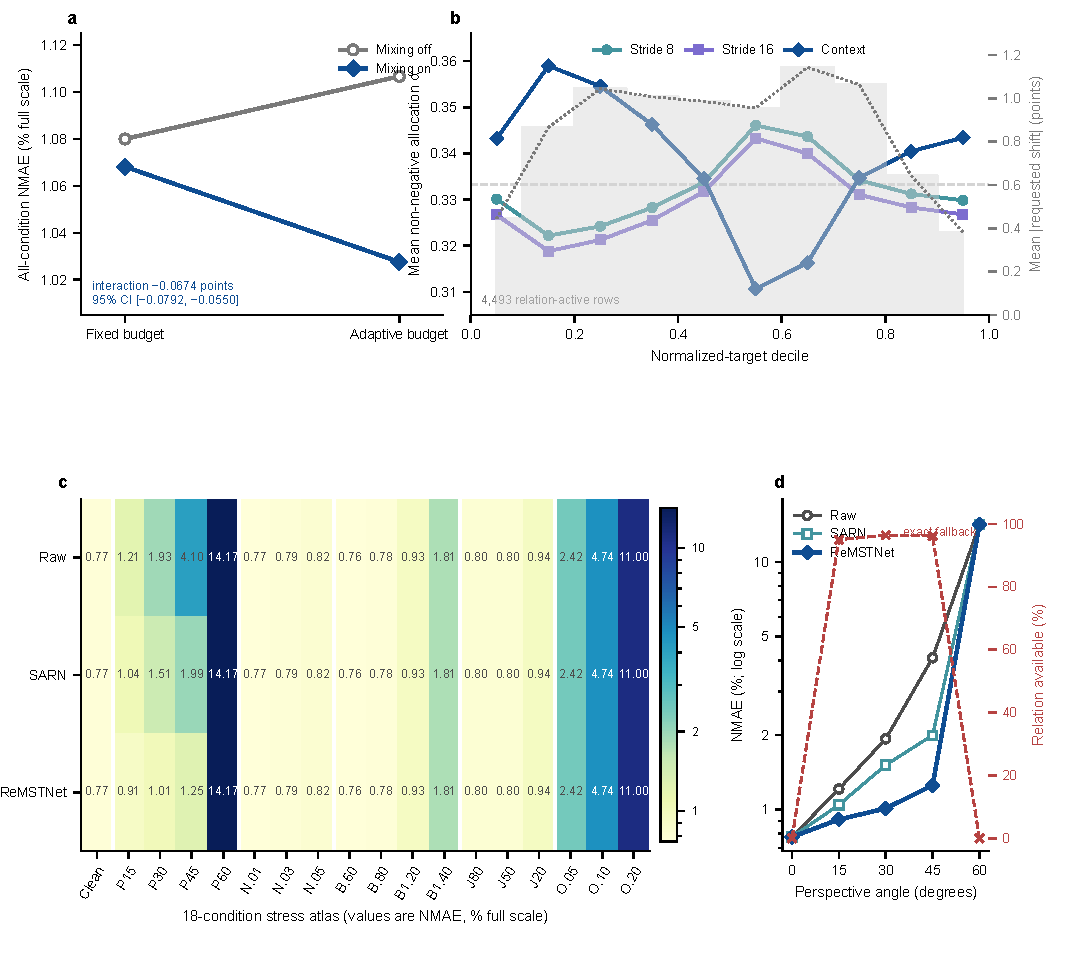
\includegraphics[width=\textwidth]{remstnet_mechanism_validity.pdf}
\caption{Mechanism evidence and declared validity boundary. (\textbf{a}) Fixed-seed $2\times2$ factorial comparison of progress mixing and the adaptive budget, with the all-condition difference-in-differences interval. (\textbf{b}) Mean non-negative allocation among stride-8, stride-16, and context transport stages across normalized-target deciles, together with the mean absolute requested shift. This panel contains 4493 relation-active projective rows from source seed 20262022. (\textbf{c}) Single-seed 18-condition stress atlas for Raw, SARN, and \modelname; cell values are NMAE as a percentage of full scale and color is logarithmic. (\textbf{d}) Perspective subset with relation availability on the secondary axis. The relation is available for approximately 95--96\% of rows at 15--$45^{\circ}$ and unavailable at $60^{\circ}$, where all outputs return exactly to the Raw endpoint.}
\label{fig:mechanism_validity}
\end{figure}

\subsection{Natural-Repeat Stability}
\label{subsec:repeat_results}

The natural-repeat cohort comprised 1,203 images, 86 complete repeat units, and 31 physical-gauge groups. Coverage was 100\% for every seed. \modelname\ obtained full-denominator NMAE $0.115867\pm0.017559$, mean within-unit population standard deviation $0.040791\pm0.003272$, and mean within-unit range $0.143147\pm0.013271$. Because the protocol used clean images and the relation was inactive, \modelname, SARN, and Raw were exactly equal row by row; every paired difference and physical-group bootstrap interval was zero. The experiment therefore shows preservation, not improvement, of clean repeat stability.

\subsection{Parameters and CUDA Efficiency}
\label{subsec:efficiency_results}

The parameter and latency results are summarized in Table~\ref{tab:efficiency}. The Raw foundation and twin endpoint share weights and therefore have the same unique parameter count, although the latter executes the foundation twice. \modelname\ adds 261,528 trainable relation parameters, increasing the unique count by 6.52\% relative to the twin endpoint.

\begin{table}[H]
\caption{Matched BF16 efficiency on an NVIDIA GeForce RTX 4060. B8 latency is reported per sample. SARN materialization was outside the timed region.}
\label{tab:efficiency}
\centering
\resizebox{\textwidth}{!}{%
\begin{tabular}{lcccccc}
\toprule
\textbf{Arm} & \textbf{Unique params.} & \textbf{ReMST-trainable} & \textbf{B1 mean/P50/P95 (ms)} & \textbf{B8 ms/sample} & \textbf{B8 samples/s} & \textbf{Peak B1/B8 (MiB)} \\
\midrule
Raw foundation & 4.010M & 0 & 7.973/7.834/9.635 & 1.123 & 890.82 & 30.9/81.7 \\
Raw+SARN twin endpoint & 4.010M & 0 & 14.551/14.506/15.142 & 2.118 & 472.25 & 31.8/88.7 \\
\modelname-v3 & 4.272M & 0.262M & 30.640/30.596/31.969 & 4.138 & 241.67 & 34.2/94.9 \\
\bottomrule
\end{tabular}}
\end{table}

At batch size 1, \modelname\ added 16.09~ms relative to the twin endpoint and processed 32.64 samples/s. At batch size 8 it processed 241.67 samples/s. These measurements characterize ROI-model execution, not camera-to-API latency. FLOPs are not reported because the available dispatcher did not count the custom Newton solver and grid-sampling path completely; reporting a partial count would understate the executed computation.

\subsection{Supplementary Diagnostics and Qualitative Cases}
\label{subsec:supplementary_figures}

The following supplementary figures expose training-seed variation, repeat dispersion, the accuracy--latency trade-off, the full error tail, and objectively selected public examples. They are included to make heterogeneity and failure behavior inspectable rather than to add new hypothesis tests.

\setcounter{figure}{0}
\renewcommand{\thefigure}{S\arabic{figure}}

\begin{figure}[H]
\centering
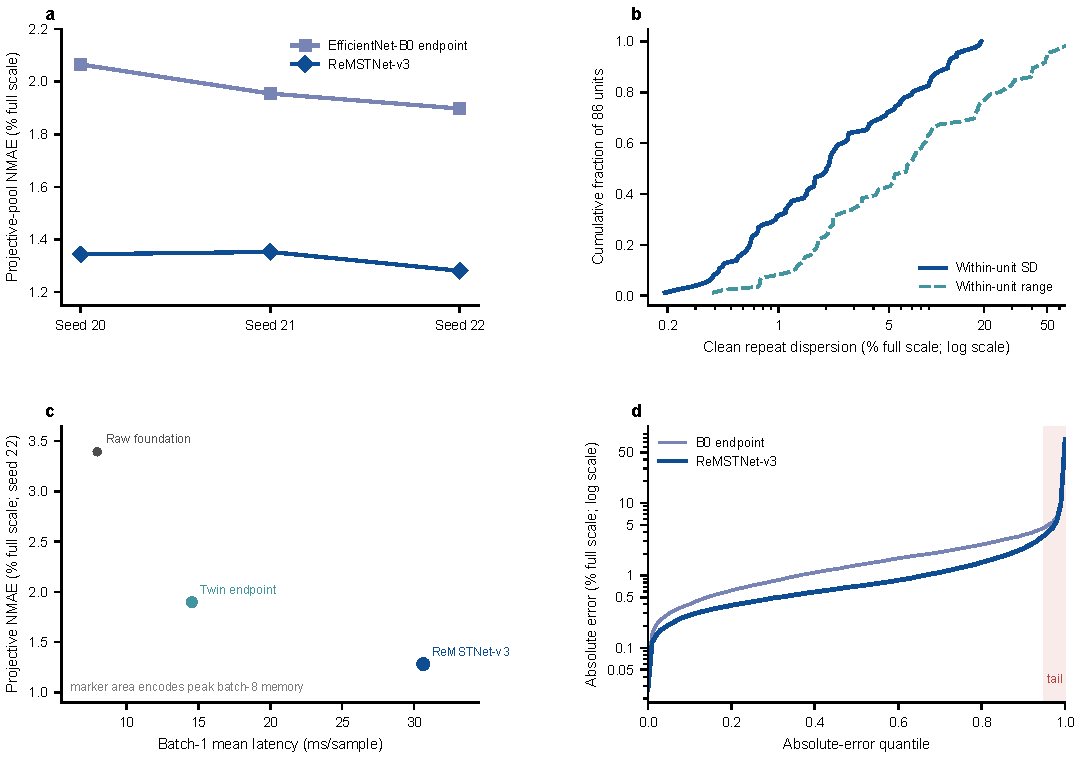
\includegraphics[width=\textwidth]{remstnet_supp_diagnostics.pdf}
\caption{Seed, repeatability, efficiency, and tail diagnostics. (\textbf{a}) Projective-pool NMAE for the seed-matched EfficientNet-B0 endpoint and \modelname\ in each of the three independently trained runs. (\textbf{b}) Empirical cumulative distributions of within-repeat-unit population SD and range for 86 complete natural-repeat units; each unit-level statistic was averaged across seeds. (\textbf{c}) Batch-1 mean latency versus projective NMAE for source seed 20262022; marker area encodes peak batch-8 memory. SARN materialization was outside the timed region. (\textbf{d}) Projective-row absolute-error quantile functions after row-wise averaging across the three seeds; the shaded region marks the upper 5\% tail.}
\label{fig:supp_diagnostics}
\end{figure}

\begin{figure}[H]
\centering
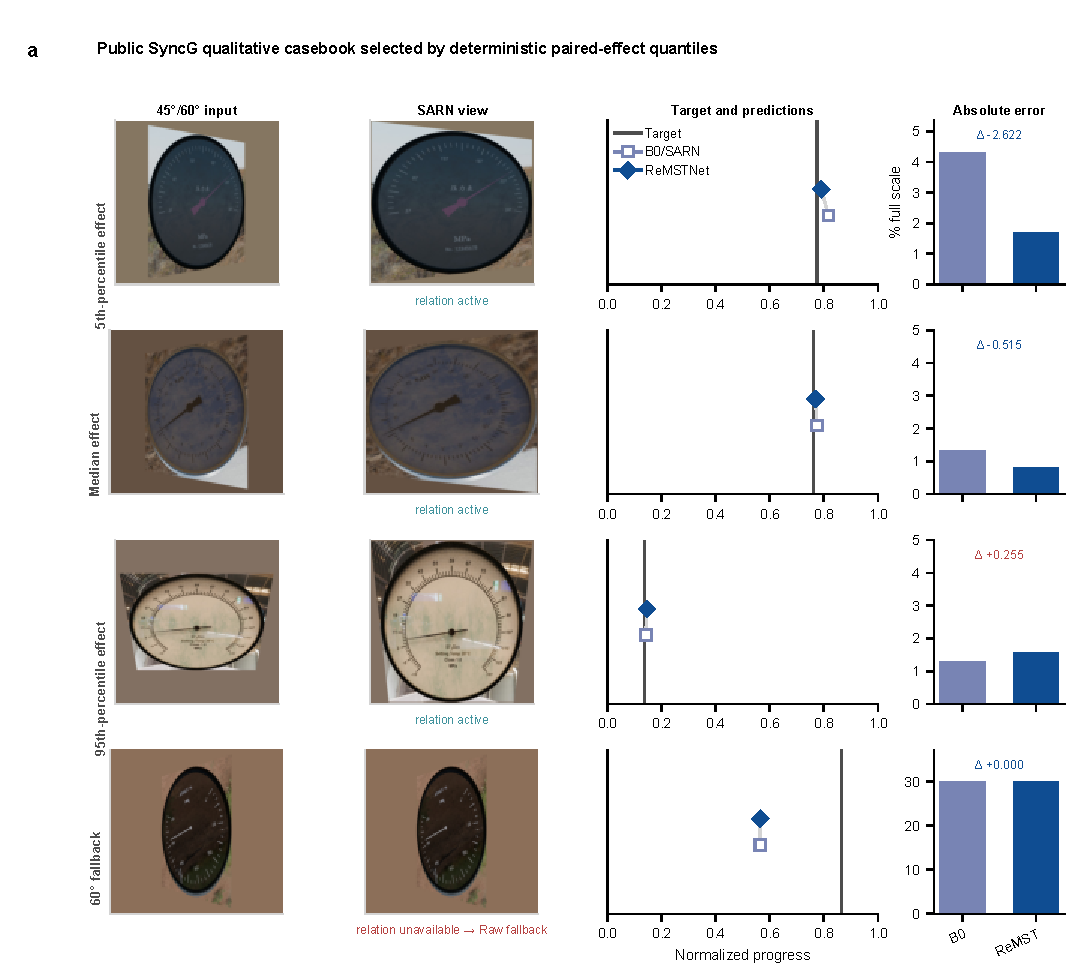
\includegraphics[width=\textwidth]{remstnet_supp_casebook.pdf}
\caption{Public SyncG qualitative casebook with objective selection and an explicit fallback. The first three rows are the 5th-, 50th-, and 95th-percentile paired changes in absolute error among relation-active $45^{\circ}$ rows after row-wise averaging across the three seeds. From left to right, each row shows the transformed input, SARN view, target and predictions, and endpoint versus \modelname\ absolute error. The 95th-percentile row retains a visible negative-transfer case rather than selecting only favorable examples. The last row applies the fixed $60^{\circ}$ stress transform to the Figure~\ref{fig:task_scope} example; relation validation fails, the SARN view is a no-op, and the endpoint and \modelname\ errors are exactly equal. The quantile rule is deterministic, and the images are illustrative rather than inferential evidence.}
\label{fig:supp_casebook}
\end{figure}

\section{Discussion}
\label{sec:discussion}

The central result is condition-specific rather than universal. \modelname\ left the seed-matched EfficientNet-B0 endpoint unchanged on clean and blur-only inputs at displayed precision, but substantially reduced error once a valid projective-support relation was available. This pattern agrees with the architecture: the model receives no license to modify an image merely because it is difficult. It may transport the endpoint only after SARN identifies a supported crop and both hierarchical alignments remain valid. The 18-condition negatives and the $60^{\circ}$ fallback are therefore as important as the 15--$45^{\circ}$ gains.

The mechanism experiment refines that interpretation. A learnable budget was not independently beneficial in this run; without local progress mixing, enabling it worsened NMAE. Mixing neighboring bins produced a small improvement on its own and changed the estimated effect of the budget from harmful to favorable. The negative interaction interval is consistent with the proposed sequence: local mixing first organizes adjacent-bin evidence, after which the bounded gain scales the permitted first-moment movement. This factorial contrast is more informative about the combined design than four isolated point estimates, but it remains a fixed-seed result whose interval excludes retraining variation.

Moment-constrained transport supplies a useful functional restriction. Unconstrained scalar correction can change a reading without preserving a defined relationship to the source distribution. Equations~\eqref{eq:feasible_target}--\eqref{eq:exponential_tilt} instead produce the minimum-KL distribution whose first moment matches the feasible clipped target to numerical tolerance, while the simplex allocation prevents requested opposite-sign stage corrections. When clipping is inactive, the requested shifts telescope to $\Delta$; near a progress boundary, the realized movement can be smaller. Exact zero-shift endpoint and invalid-relation Raw fallback make equivalence testable at the prediction level. These properties do not guarantee correctness: a valid-looking but misleading support can still yield an erroneous correction, and the fallback checks geometry rather than model error. They constrain how a correction occurs, not whether its target is always right.

The comparison with existing gauge readers also requires attention to system boundaries. Perspective-correction pipelines may explicitly rectify a dial before segmentation \cite{tan2024transunet}, incorporate route and range priors \cite{chu2025prikmet}, or infer virtual points for strong pose correction \cite{lee2026p2yolo}. Vector and reconstruction approaches address pointer representation or occlusion \cite{dong2021vdn,ninama2026grnet}. The core \modelname\ method receives an already cropped single-pointer ROI and a pixel-derived support normalization, then refines normalized progress. Table~\ref{tab:vdn_intersection} covers identical pixels but gives VDN annotation-derived pivot and ordered scale endpoints for offline conversion, so it is a component comparison rather than an automatic-system ranking. The RPM-10K track disables relation input and is likewise not a relation comparison. Section~\ref{subsec:ocr_e2e_results} is the only track that converts an automatically recovered range and normalized progress into physical units. It integrates existing OCR, is selective, and replays cached boxes; its conditional NMAE therefore must not be substituted for the full-denominator result or directly ranked against prospectively measured acquisition-to-reading systems.

The unified industrial result strengthens the transfer evidence beyond separate source-cohort point estimates. Its 1,395 ROIs exactly match the organized real-photo benchmark, the six-condition and projective-pool intervals are below zero, and all three projective conditions favor \modelname. The absolute effects remain modest, but their condition specificity is the intended signature of selective transport: clean and blur-only photographs preserve the endpoint, whereas supported projective views are corrected. These controlled support-generating transforms do not solve natural-viewpoint estimation. RPM-10K exposes a raw-foundation domain gap, but because its protocol disables relation input it cannot determine whether a natural-geometry extension of \modelname\ would improve that dataset.

The two full-frame replays answer different deployment questions. The scalar path confirms that the repository's industrial \texttt{data/} photographs, after deduplication into the organized deployment roster, can cross the cached detector-to-reader boundary with 98.69\% coverage and measurable normalized-progress accuracy on the labeled subset. The independent OCR execution goes one system stage further: PP-OCRv4 and production point geometry yield physical readings for 17.65\% of all photographs and 27.27\% of labeled photographs. On those accepted labeled frames, automatic range recovery adds only $0.002478\pm0.002546$ NMAE relative to the matched true-range calculation, but the full-denominator result remains poor because most photographs do not produce a range. Neither replay supplies an independent cohort: these photographs underlie the 1,395 ROI baseline, only 33 full frames have compatible physical labels, and cached detections cannot establish detector recall or localization quality without box truth. The industrial sources were retrospectively evaluated after engineering exposure, the External-ROI identities remain provisional, and RF100-derived is a small non-leaderboard cohort. A prospective multi-site study with verified instrument groups and independently acquired ground truth is still needed.

The computational trade-off is moderate in parameters but noticeable in execution. Relation modules add only 6.52\% unique parameters to the shared twin endpoint, but two-view encoding, feature alignment, attention, and three Newton projections more than double batch-1 latency relative to that endpoint. The measured 32.64 samples/s is a model-only throughput result; the benchmark excludes image decoding and SARN materialization and was not compared with a stated application deadline. Deployment suitability must therefore be assessed with a complete acquisition-to-result profile and an explicit latency requirement on the target device rather than inferred from Table~\ref{tab:efficiency} alone.

Several additional limitations remain. First, the learned reader covers one pointer and normally assumes a known ROI. The full-frame replays expose detector and OCR/range failures but use cached boxes without bounding-box truth. Existing-model physical-unit conversion is demonstrated only selectively: the default range decoder returns 27/153 outputs and robust multiple-pointer handling, low-contrast numeral recognition, and reliable range inference remain unresolved. Second, SARN-v2 recognizes a particular padded projective-support pattern and was inactive on RPM-10K and native clean industrial photographs, so it does not yet correct arbitrary natural obliquity or generic blur. Third, the 128-bin posterior uses a fixed scale, so CRPS, coverage, PIT, or variance should not be reported as calibrated uncertainty without a separate calibration study. Fourth, first-moment constraints do not resolve multimodal semantic ambiguity, such as confusing the pointer with a scale mark. Fifth, only the relation modules were fitted for five epochs while the imported foundation remained frozen; larger-scale joint training and other foundation families may change the accuracy--latency balance. Sixth, the Scene-Holdout roster is scene-disjoint from fitting but has been reused for project-level method comparison, so it provides retrospective development evidence rather than untouched confirmation. Seventh, the VDN comparison contains six scene groups and one checkpoint and uses annotation-derived reference geometry; it is not an automatic-system comparison and omits VDN retraining uncertainty. Eighth, RPM-10K's upstream dataset license remains unspecified, the industrial benchmark is retrospective rather than blind, and only 33 full frames have compatible physical labels. Future work should learn support and homography evidence from natural multi-view data, improve OCR and automatic-range coverage under blur, glare, low contrast, and oblique views, calibrate predictive distributions, and validate the complete live acquisition-to-physical-reading pipeline prospectively across instruments, sites, cameras, and acquisition angles.

\section{Conclusions}
\label{sec:conclusions}

This study introduced \modelname, a hierarchical dual-view network for normalized pointer-gauge progress under a defined projective-support relation. Two relation blocks rewrite intermediate Raw features using aligned SARN evidence, and a progress-aware coordinator converts multi-scale relations into a bounded set of same-sign requested shifts. Sequential information projections match feasible clipped first-moment targets to numerical tolerance, while invalid geometry returns the Raw posterior exactly.

Across three independent SyncG runs, \modelname\ achieved $0.010704\pm0.000373$ all-condition NMAE and $0.013259\pm0.000391$ projective-pool NMAE, improving over three matched lightweight architecture baselines in the aggregate. On the complete 774-row same-pixel VDN intersection, \modelname\ obtained $0.008582\pm0.000414$ versus 0.016444 NMAE for the annotation-assisted VDN reference, a 47.81\% reduction; the projective reduction was 47.99\%. On the exact 1,395-ROI industrial real-photo baseline, the six-condition paired interval, projective-pool interval, and all three individual projective-condition intervals favored \modelname. Direct full-frame use of the organized deployment photographs yielded 151/153 scalar detector/read coverage and $0.051930\pm0.001031$ NMAE on 33 labeled frames. A separate PP-OCRv4 integration produced physical readings for 27/153 photographs; on the nine labeled photographs accepted by the default decoder, conditional NMAE was $0.036814\pm0.004015$ versus $0.034336\pm0.003848$ with matched true ranges. RPM-10K remains a raw-foundation diagnostic because its released protocol disables relation inputs. Together with the factorial, stress, and repeat controls, these results establish relation-conditioned posterior transport as a selective projective correction on synthetic and industrial photographs and demonstrate feasible existing-model physical-unit integration on accepted frames. They do not establish arbitrary natural-viewpoint correction, a validated live detector, or high-coverage OCR-complete industrial reading.

\vspace{6pt}

% Required before submission: uncomment and complete after the author confirms
% the applicable CRediT roles and funding status.
% \authorcontributions{Conceptualization, X.L.; methodology, X.L.; ...}
% \funding{This research received no external funding.}

\institutionalreview{Not applicable.}

\informedconsent{Not applicable.}

\dataavailability{SyncG, RPM-10K, and the RF100-derived source are identified in their cited releases. RPM-10K was used only for local evaluation; its upstream repository currently lists the dataset license as ``TBD'', so its images, labels, and derived manifest are not redistributed. The RF100-derived source is the \emph{needle-base-tip-min-max} test subset at \url{https://universe.roboflow.com/rf-100-vl/needle-base-tip-min-max-u87vi-wzsrt-kjyu}. The industrial ROI baseline and full-frame diagnostics are organized locally as \texttt{unified\_real\_photo\_progress\_v1} from project deployment photographs in \texttt{data/} and \texttt{data-717/}; the full collection is not publicly redistributed because release remains subject to project permissions. The two detector crops in Figure~\ref{fig:ocr_e2e} are included only as illustrative manuscript panels. Source code, OCR evaluation code, aggregate JSON, and figure source CSV files are included with the project release, while remaining raw external and industrial data remain excluded.}

\acknowledgments{During the preparation of this manuscript, the author used OpenAI Codex (accessed 21 August 2026) for assistance with manuscript drafting, generation of figure source code, and consistency inspection of source code and stored aggregate result files. The author reviewed and edited the output and takes full responsibility for the content of this publication.}

% Required before submission: uncomment after the author confirms the conflict-of-interest status.
% \conflictsofinterest{The author declares no conflict of interest.}

\abbreviations{Abbreviations}{%
The following abbreviations are used in this manuscript:\\

\noindent
\begin{tabular}{@{}ll}
BF16 & Brain floating-point format\\
CDF & Cumulative distribution function\\
CRPS & Continuous ranked probability score\\
CVaR & Conditional value at risk\\
H2D & Host-to-device\\
KL & Kullback--Leibler\\
NMAE & Normalized mean absolute error\\
OCR & Optical character recognition\\
ONNX & Open Neural Network Exchange\\
PIT & Probability integral transform\\
ReMST & Relation-encoded moment-exact scalar transport\\
RMSE & Root mean squared error\\
ROI & Region of interest\\
SARN & Support-aware ROI normalization
\end{tabular}
}

\begin{adjustwidth}{-\extralength}{0cm}
\reftitle{References}
\bibliography{references}
% Publisher production text; MDPI will insert this if needed after acceptance.
% \PublishersNote{}
\end{adjustwidth}

\end{document}
